\documentclass[russian, 12pt]{beamer}
\usepackage{multicol}
\usepackage[T2A,T1]{fontenc}
\usepackage[utf8]{inputenc}
\setcounter{secnumdepth}{3}
\setcounter{tocdepth}{3}
\usepackage{amsmath}
\usepackage{amssymb}
\usepackage{graphicx}
\usepackage{paratype}
\usepackage{hyperref}
\usepackage{xcolor}
\usepackage{listings}

\definecolor{codegreen}{rgb}{0,0.6,0}
\definecolor{codegray}{rgb}{0.5,0.5,0.5}
\definecolor{codepurple}{rgb}{0.58,0,0.82}
\definecolor{backcolour}{rgb}{0.95,0.95,0.92}

\lstdefinestyle{mystyle}{
    backgroundcolor=\color{backcolour},   
    commentstyle=\color{codegreen},
    keywordstyle=\color{magenta},
    numberstyle=\tiny\color{codegray},
    stringstyle=\color{codepurple},
    basicstyle=\ttfamily\footnotesize,
    breakatwhitespace=false,         
    breaklines=true,                 
    captionpos=b,                    
    keepspaces=true,                 
    numbers=left,                    
    numbersep=5pt,                  
    showspaces=false,                
    showstringspaces=false,
    showtabs=false,                  
    tabsize=2
}

\newcommand{\R}{\mathbb{R}}
\newcommand{\A}{\mathcal{A}}
\newcommand{\red}[1]{\textcolor{red!85!black}{{#1}}}
\renewcommand{\sp}[1]{\mathrm{sp}\left\{{{#1}}\right\}}
% Syntax: \colorboxed[<color model>]{<color specification>}{<math formula>}
\newcommand*{\colorboxed}{}
\def\colorboxed#1#{%
  \colorboxedAux{#1}%
} 
\newcommand*{\colorboxedAux}[3]{%
  % #1: optional argument for color model
  % #2: color specification
  % #3: formula
  \begingroup
    \colorlet{cb@saved}{.}%
    \color#1{#2}%
    \boxed{%
      \color{cb@saved}%
      #3%
    }%
  \endgroup
}

\makeatletter
\usepackage{tikz}
\usetikzlibrary{overlay-beamer-styles}
\usepackage{pgfplots}
% Remove warning about running in backwards compatibility mode
\pgfplotsset{compat=1.17}
\usepackage[all,cmtip]{xy}
\usetheme{Pittsburgh}
\usefonttheme{professionalfonts}

\setbeamertemplate{navigation symbols}{%
  \hspace{3.8em}%
  \vspace{0.5em}%
  \usebeamercolor[fg]{structure}%
  \usebeamerfont{subtitle}%
  \insertframenumber%
}
\makeatother
\setbeamercovered{invisible}

\usepackage{babel}

\title{Алгоритмы поиска. Оценка сложности.}
\subtitle{Алгоритмы и структуры данных}
\author{
  Мулюгин Николай
  %\and
  %Кузнецов Максим \texorpdfstring{\thinspace}{Lg}А.
  }
\date{10.09.2022}

\begin{document}

\begin{frame}
\titlepage
\end{frame}

%%%%%%%%%%%%%%%%%%%%%%%%%%%%%%%%%%%%%%%%%%%%%%%%%%%%%%%%%%%%%%%%%%%%%%%%%%%%%%%
\begin{frame}
\frametitle{Мотивация}
  \begin{itemize}
    \item Зачем нам что то искать?\\[0.5cm]
    \pause
    \item Зачем нам что то быстро искать?\\[0.5cm]
    \pause
    \item Где нам искать?\\[0.5cm]
    
    %\item Повседневное применение.\\[0.5cm]

  \end{itemize}
\end{frame}
%%%%%%%%%%%%%%%%%%%%%%%%%%%%%%%%%%%%%%%%%%%%%%%%%%%%%%%%%%%%%%%%%%%%%%%%%%%%%%%
\begin{frame}
\frametitle{Массив}
\begin{center}
  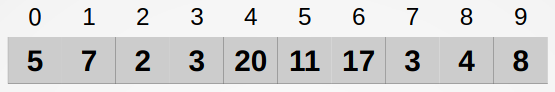
\includegraphics[scale=0.5]{img/array.png}\\  
\end{center}\pause
  \textbf{Массив} - структура данных, хранящая набор значений 
  в памяти непосредственно друг за другом\\[0.3cm]\pause
  \textbf{Индекс массива} - номер элемента в массиве 
  в памяти непосред\\[0.3cm]\pause
  Вопрос: сложно ли получить элемент по индексу?\\ \pause
  Ответ: \;$O(1)$
\end{frame}
%%%%%%%%%%%%%%%%%%%%%%%%%%%%%%%%%%%%%%%%%%%%%%%%%%%%%%%%%%%%%%%%%%%%%%%%%%%%%%%
\lstset{style=mystyle}
\begin{frame}[fragile]
\frametitle{Массив}
\begin{center}
  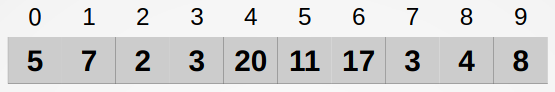
\includegraphics[scale=0.5]{img/array.png}\\  
\end{center}
Массивы в C++
\begin{lstlisting}[language=C++]
//create array with 4 int type elements
int[4] arr = {5,7,2,3};
//read value at 3
int three = arr[3];//three = 3
//write to 3
arr[3] = 4;//[5 7 2 4]
\end{lstlisting}
\end{frame}
%%%%%%%%%%%%%%%%%%%%%%%%%%%%%%%%%%%%%%%%%%%%%%%%%%%%%%%%%%%%%%%%%%%%%%%%%%%%%%%
\lstset{style=mystyle}
\begin{frame}[fragile]
\frametitle{Линейный поиск}
\begin{lstlisting}[language=C++]
int LinearSearch1( int* arr, int n, int x)
{
  int answer = -1;
  for( int i = 0; i < n; i++ )
    if(arr[i] == x)
      answer = i;
  return answer;
}
\end{lstlisting}
$\text{f(n)} = \pause(C_{=} + C_{<} + C_{+} + C_{==} + C_{=} ) \cdot n 
= C \cdot n$\\[0.3cm] \pause
$\boxed{\text{f(n)} = \Theta (n)}$
\end{frame}
%%%%%%%%%%%%%%%%%%%%%%%%%%%%%%%%%%%%%%%%%%%%%%%%%%%%%%%%%%%%%%%%%%%%%%%%%%%%%%%
\lstset{style=mystyle}
\begin{frame}[fragile]
\frametitle{Линейный поиск}
\begin{lstlisting}[language=C++]
int LinearSearch2( int* arr, int n, int x)
{
  for( int i = 0; i < n; i++ )
    if(arr[i] == x)
      return i;
  return -1;
}
\end{lstlisting}
\end{frame}
%%%%%%%%%%%%%%%%%%%%%%%%%%%%%%%%%%%%%%%%%%%%%%%%%%%%%%%%%%%%%%%%%%%%%%%%%%%%%%%
\lstset{style=mystyle}
\begin{frame}[fragile]
\frametitle{Бинарный поиск}
\begin{lstlisting}[language=C++]
//sorted array 2 5 6 15 21 23 25
int BinarySearch(int* arr, int n, int key) {
  int low = 0;
  int high = n - 1;

  while (low <= high) {
      int mid = (low + high) / 2;
      int midVal = arr[mid];

      if (midVal < key)
          low = mid + 1;
      else if (midVal > key)
          high = mid - 1;
      else
          return mid; // key found
  }
  return -(low + 1);  // key not found.
}
\end{lstlisting}
\end{frame}
%%%%%%%%%%%%%%%%%%%%%%%%%%%%%%%%%%%%%%%%%%%%%%%%%%%%%%%%%%%%%%%%%%%%%%%%%%%%%%%
\begin{frame}[fragile]
Сложность бинарного поиска f(n) = ?\pause
\begin{lstlisting}[language=C++]
int[7] arr = { 2,5,6,15,21,23,25 };
int* arr_ptr = &arr[0];
int n = 7;
int ans_i = BinarySearch( arr_ptr, n, 2 );   
\end{lstlisting}
\begin{center}
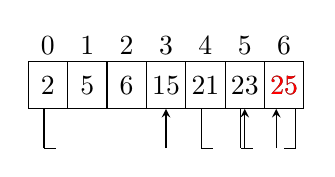
\begin{tikzpicture}
  \draw<-6> (-2.75, 0.8) node[scale=1, ] {0};
  \draw<-6> (-2.75, 0.3) node[scale=1, ] {2};
  \draw<-6> (-3,0) rectangle (-2.5, 0.6);

  \draw<-6> (-2.25, 0.8) node[scale=1, ] {1};
  \draw<-6> (-2.25, 0.3) node[scale=1, ] {5};
  \draw<-6> (-2.5,0) rectangle (-2, 0.6);

  \draw<-6> (-1.75, 0.8) node[scale=1, ] {2};
  \draw<-6> (-1.75, 0.3) node[scale=1, ] {6};
  \draw<-6> (-2,0) rectangle (-1.5, 0.6);

  \draw<-6> (-1.25, 0.8) node[scale=1, ] {3};
  \draw<-6> (-1.25, 0.3) node[scale=1, ] {15};
  \draw<-6> (-1.5,0) rectangle (-1, 0.6);

  \draw<-6> (-0.75, 0.8) node[scale=1, ] {4};
  \draw<-6> (-0.75, 0.3) node[scale=1, ] {21};
  \draw<-6> (-1,0) rectangle (-0.5, 0.6);

  \draw<-6> (-0.25, 0.8) node[scale=1, ] {5};
  \draw<-6> (-0.25, 0.3) node[scale=1, ] {23};
  \draw<-6> (-0.5,0) rectangle (0, 0.6);

  \draw<-6> (0.25, 0.8) node[scale=1, ] {6};
  \draw<1> (0.25, 0.3) node[scale=1, ] {25};
  \draw<2-6> (0.25, 0.3) node[scale=1, color=red] {25};
  \draw (0,0) rectangle (0.5, 0.6);
  
  \draw<2-6> (0.4, 0) -- (0.4, -0.5);
  \draw<2-6> (0.25, -0.5) -- (0.4, -0.5);

  \draw<2-3> (-2.8, 0) -- (-2.8, -0.5);
  \draw<2-3> (-2.8, -0.5) -- (-2.65, -0.5);

  \draw<3-4>[-stealth] (-1.25, -0.5) -- (-1.25, 0);

  \draw<4-5> (-0.8, 0) -- (-0.8, -0.5);
  \draw<4-5> (-0.8, -0.5) -- (-0.65, -0.5);
  \draw<5>[-stealth] (-0.25, -0.5) -- (-0.25, 0);

  \draw<6> (-0.3, 0) -- (-0.3, -0.5);
  \draw<6> (-0.3, -0.5) -- (-0.15, -0.5);
  \draw<6>[-stealth] (0.15, -0.5) -- (0.15, 0);

\end{tikzpicture}
\end{center}

\end{frame}
%%%%%%%%%%%%%%%%%%%%%%%%%%%%%%%%%%%%%%%%%%%%%%%%%%%%%%%%%%%%%%%%%%%%%%%%%%%%%%%
\begin{frame}[fragile]
\frametitle{Сложность бинарного поиска}
Сложность бинарного поиска f(n) = ?\\[0.3cm] \pause
$0\; 1\; 2\; 3\; 4\; 5\; 6\; \dots\dots\dots\dots\dots\dots \; n\left(\frac{n}{2^1}\right) $\\[0.3cm] \pause
$0\; 1\; 2\; 3\; 4\; 5\; 6\; \dots\dots\dots \;\frac{n}{2}\left(\frac{n}{2^1}\right)\dots$\\[0.3cm] \pause
$0\; 1\; 2\; 3\; 4\; 5\; 6\; \dots \frac{n}{4}\left(\frac{n}{2^2}\right)\dots\dots$\\[0.3cm] \
$0\;\frac{n}{2^y}\dots\dots\dots$\\[0.3cm] \pause
$\frac{n}{2^y} = 1;$\pause
$\;\;n = 2^y;$\pause
$\;\;y = ?;$\pause
$\;\;\boxed{y = \log_2n}$\\[0.3cm]\pause
$\boxed{\text{f(n)} = \Theta(\log_2n)}$
%%%%%%%%%%%%%%%%%%%%%%%%%%%%%%%%%%%%%%%%%%%%%%%%%%%%%%%%%%%%%%%%%%%%%%%%%%%%%%%
\end{frame}
\begin{frame}
\frametitle{Домашнее задание}
\begin{itemize}
  \item Написать программу реализующую алгоритм Эратосфена.
  \item Оценить сложность - написать в программе комментариями мысли и результат.
  \item Сделать pull request в папку lecture$\_$01/homework/ с файлом решения.
\end{itemize}
\end{frame}


\end{document}
